% This is not necessarily in the format for a VUW thesis chapter.

% Finished July 18, 2013


\documentclass[a4paper]{report}

\usepackage{amssymb, amsmath}
%\usepackage{mathtools}
\usepackage{tikz}
\usetikzlibrary{calc}

%\usepackage{marvosym}

\newcommand{\beff}{\ensuremath{b_{\mathrm{eff}}}}
\newcommand{\bhom}{\ensuremath{b_{\mathrm{hom}}}}

\title{Chapter 6: The Homogenized Effective Slip Length}
\author{Nat Lund}


\begin{document}
\maketitle

We shall find the \emph{homogenized slip length} of a bulk of fluid flowing over a rough slippery surface.  In our mathematical model of the system,
fluid flow at each point in the bulk obeys Stokes equation:
\begin{equation}
\mu \nabla^2 \vec{u} = \nabla p
\end{equation}
And fluid at each point on the boundary satisfies the generalized slip boundary condition:
\begin{equation}
\vec{u} = b \, (\nabla \vec{u} + \nabla \vec{u}^T) \cdot \vec{n}
\end{equation}

The boundary itself roughly coincides with the $x,y$ plane. The boundary is a surface described by a height function $h(x,y)$ on the $x,y$ plane.  The $z$ direction is roughly perpendicular to the boundary, and the fluid may be supposed to be flowing in the $x$ direction. 

\begin{center}
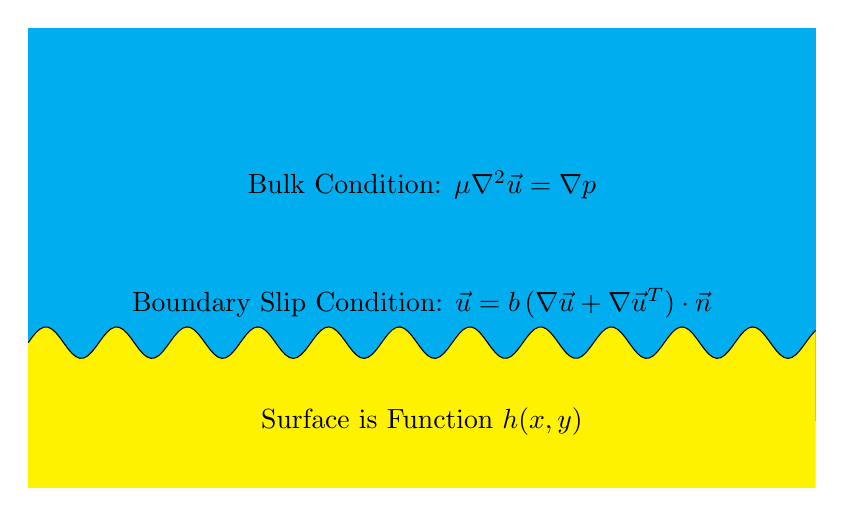
\begin{tikzpicture}
\fill[color=cyan] (0,-1) rectangle (10,4);

\node at (5,2) {Bulk Condition: $\mu \nabla^2 \vec{u} = \nabla p$};
\node at (5,0.5){Boundary Slip Condition:  $\vec{u} = b \, (\nabla \vec{u} + \nabla \vec{u}^T) \cdot \vec{n}$};

\fill [color=yellow,domain=0:10,samples=200] plot (\x,{ 0.2 * sin(7*\x r)} ) -- ++(0,-2) -| (0,0);
\draw [domain=0:10,samples=200] plot (\x,{ 0.2 * sin(7*\x r)} );

\node at (5,-1) {Surface is Function $h(x,y)$};

\end{tikzpicture}
\end{center}

The \emph{effective} slip length of a rough surface was defined back in Chapter 1.  At sufficient height above the surface, perturbations due to the rough surface have died away, and the flow \emph{behaves like} flow in an \emph{effective system:} flow over a flat `effective' surface with a uniform slip length, $\beff$. We illustrate this with Couette-type flow:

\begin{center}
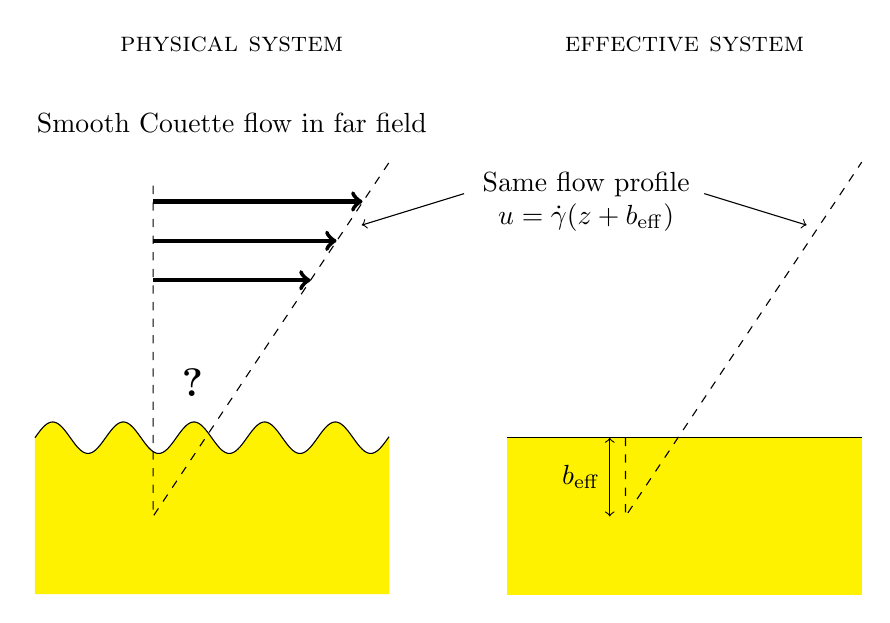
\begin{tikzpicture}

\coordinate (ori) at (0,0);
%\fill[color=cyan] (ori) ++(0,-1) rectangle ++(4.5,5);
\fill [color=yellow,domain=0:4.5,samples=200] plot (\x,{ 0.2 * sin(7*\x r)} ) -- ++(0,-2) -| (ori);
\draw [domain=0:4.5,samples=200] plot (\x,{ 0.2 * sin(7*\x r)} );

\draw[dashed] (ori) ++(1.5,3.2) -- ++(0,-4.2) -- ++(3,4.5);
\draw[->, ultra thick] (ori) ++(1.5,2) -- ++(2,0);
\draw[->, ultra thick] (ori) ++(1.5,2.5) -- ++(2.33,0);
\draw[->, ultra thick] (ori) ++(1.5,3) -- ++(2.66,0);
\node at (2,0.7) {\Large{\textbf{?}}};
\node at (2.5,4) {Smooth Couette flow in far field};


\coordinate (ori) at (6,0);
%\fill[color=cyan] (ori) ++(0,-1) rectangle ++(4.5,5);
\fill[color=yellow] (ori) rectangle ++(4.5,-2);
\draw (ori) -- ++(4.5,0);

\draw[dashed] (ori) ++(1.5,0) -- ++(0,-1) -- ++(3,4.5);
\draw[<->] (ori) ++(1.3,0) -- node[left] {\beff} ++(0,-1);

\draw[<-] (4.15,2.7) -- ++(1.3,0.4);
\draw[<-] (9.8,2.7) -- ++(-1.3,0.4);
\node at (7,3) [align=center] {Same flow profile\\$u = \dot{\gamma} (z + \beff)$};

\node at (2.5,5) {\textsc{physical system}};
\node at (8.25,5) {\textsc{effective system}};


\end{tikzpicture}
\end{center}


\subsubsection*{Homogenization}

Homogenization is a modern technique for solving partial differential equations, developed in the 1960s and '70s.  It began with the study of PDEs with rapidly oscillating coefficients.  
The basic idea was to identify the period of oscillation with a small parameter $\epsilon$, and to consider the limit as the period tended to zero.  Depending on the problem, one may get a solution as a series in $\epsilon$: $u = u_0 + \epsilon u_1 + \cdots$, or one may obtain a limiting PDE for which a solution can be found.
The technique can be applied to PDEs that hold on periodic structure; $\epsilon$ is the period of the structure.  Then we find an `effective' structure as the period of the structure tends to zero.  The first book describing homogenization appeared in 1978: ``Asymptotic Analysis for Periodic Structure", by Alain Bensoussan, Jacques-Louis Lions and George Papanicolaou.  

In standard homogenization techniques, it turns out to be necessary to cast the differential equations into variational or integral form.  As a consequence, in some cases it may be possible to exploit the fact that periodic functions weakly converge to their average.  (Weak convergence --- a kind of `convergence under the integral sign' --- will be defined shortly.)

The homogenized solution is an approximation to the solution for a system with a finite period.  The smaller the period, the better the approximation.



\vspace{1em}
Thus, homogenization is perfectly suited to our task.  
In order to use homogenization, we must slightly extend our mathematical model with the following assumptions:

\vspace{1em}
First of all, we must assume that our surface roughness is \textbf{periodic}.  That is, $h(x,y)$ is a periodic function.  This is reasonable, many real rough surfaces are at least quasi-periodic; there seems no loss of information by assuming that the surface is periodic.

Secondly, we must assume the the intrinsic slip length is a periodic function with the \textbf{same period as the roughness}.  Again, this is reasonable.   In many physical systems, the change in intrinsic slip length is \emph{due to} the roughness, eg. the increased slip over nanobubbles.

\vspace{1em}
Then, broadly speaking, the homogenization procedure is as follows:
The period is reduced sequentially, eg. the period is halved at each step in a sequence.
The \emph{amplitude} of the roughness must be reduced at the same rate, so that local gradient and curvature of the surface remain unchanged.  In the limit of the period tending to zero, we have the \textbf{homogenized} equations of flow, which we can consider to model a homogenized system.  The homogenized equations contain a slip length parameter.  In the language of homogenization theory, this is known as the \textbf{effective} slip length parameter.

Illustrating again with Couette-type flow:

\begin{center}
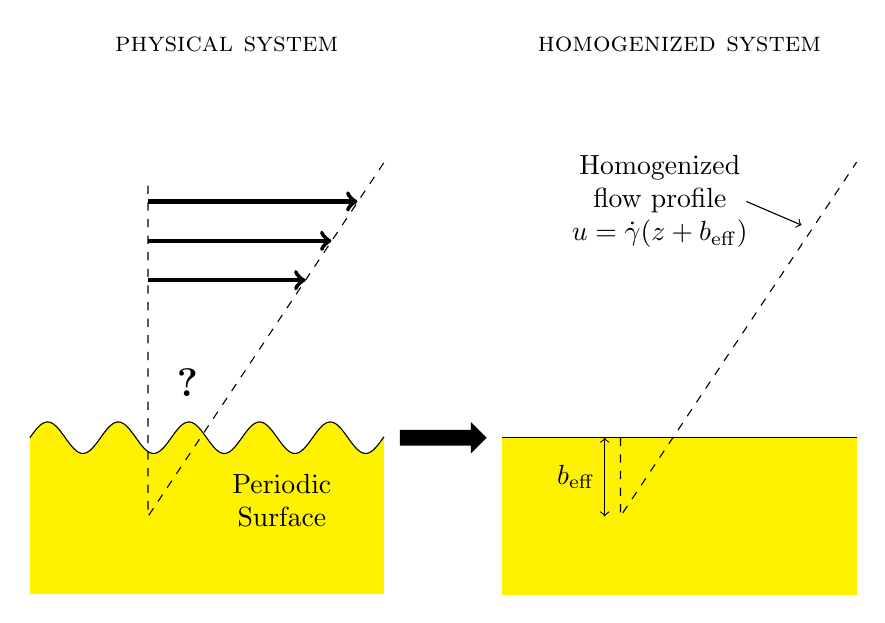
\begin{tikzpicture}

\coordinate (ori) at (0,0);
%\fill[color=cyan] (ori) ++(0,-1) rectangle ++(4.5,5);
\fill [color=yellow,domain=0:4.5,samples=200] plot (\x,{ 0.2 * sin(7*\x r)} ) -- ++(0,-2) -| (ori);
\draw [domain=0:4.5,samples=200] plot (\x,{ 0.2 * sin(7*\x r)} );

\draw[dashed] (ori) ++(1.5,3.2) -- ++(0,-4.2) -- ++(3,4.5);
\draw[->, ultra thick] (ori) ++(1.5,2) -- ++(2,0);
\draw[->, ultra thick] (ori) ++(1.5,2.5) -- ++(2.33,0);
\draw[->, ultra thick] (ori) ++(1.5,3) -- ++(2.66,0);
\node at (2,0.7) {\Large{\textbf{?}}};
\node at (3.2,-0.8)[align=center] {Periodic\\ Surface};


\coordinate (ori) at (6,0);
%\fill[color=cyan] (ori) ++(0,-1) rectangle ++(4.5,5);
\fill[color=yellow] (ori) rectangle ++(4.5,-2);
\draw (ori) -- ++(4.5,0);

\draw[dashed] (ori) ++(1.5,0) -- ++(0,-1) -- ++(3,4.5);
\draw[<->] (ori) ++(1.3,0) -- node[left] {\beff} ++(0,-1);

\draw[<-] (9.8,2.7) -- ++(-0.7,0.3);
\node at (8,3) [align=center] {Homogenized\\ flow profile\\$u = \dot{\gamma}( z + \beff)$};

\node at (2.5,5) {\textsc{physical system}};
\node at (8.25,5) {\textsc{homogenized system}};

\fill (5.8,0) -- ++(-0.2,0.2) -- ++(0,-0.1) --++(-0.9,0) -- ++(0,-0.2) -- ++(0.9,0) -- ++(0,-0.1);

\end{tikzpicture}
\end{center}

For Couette-type flow, we have defined the effective slip length as the slip length of an `effective' physical system, with flow solution $u = \dot{\gamma} (z + \beff)$.

If the same system is homogenized, the solution to the homogenized equations is $u = \dot{\gamma} (z + \beff)$.  We see immediately that the homogenized effective slip length exactly matches our physical definition of effective slip length.

\vspace{1em}
Let us now homogenize.  The particular homogenization technique we shall use comprises the following steps:

\subsubsection*{Homogenization Process Overview}

\begin{enumerate}
\item Convert the model PDEs to variational (integral) form.
\item Create a sequence of variational formulations.
\item Find the limit formulation of the sequence:
\begin{itemize}
    \item Periodic functions weakly converge to their mean;
    \item This lets us find the limit formulation.
\end{itemize}
      
\item Convert the limit formulation back to classical formulation
\item Extract the implied slip length as the \emph{homogenized} slip length.
\end{enumerate}



\subsection*{Variational Form}

The variational form comes originally from the Calculus of Variations.  The canonical use for the calculus of variations is with a \emph{minimization} problem.  We seek a \emph{function} on a domain that minimizes some quantity.  The quantity to be minimized is a \emph{functional}, a mapping from the space of functions to the real numbers.  Naturally, the functional will be some kind of integral, with the integrand being some combination of the function, its derivatives (of various order), and position in the domain.

\begin{equation}
F(u) = \int_a^b f(u,u', ...\, ,x) \; dx,  \qquad F(u) \mapsto \mathbb{R}
\end{equation} 

The boundary values of the function $u(x)$ are given.  The basic concept of calculus of variations is to take $u(x)$ to be the solution function that minimizes the functional $F$.  That being the case, any \emph{variation} away from $u$, however small, will increase $F$.  Let $v(x)$ be an arbitrary function that is zero at the boundary (i.e. zero at $a$ and $b$), and let $\epsilon$ be a small parameter. Then:

\begin{equation}
F(u) \leq F(u + \epsilon v) \qquad \forall v: v(a) = v(b) = 0
\end{equation}

\vspace{1em}

\begin{center}
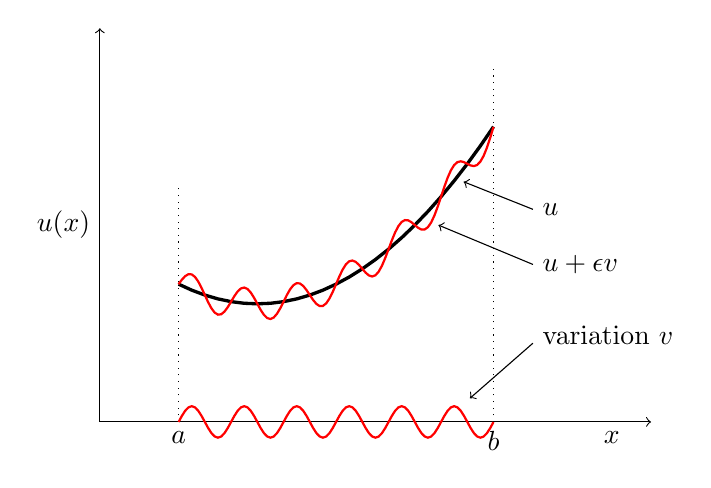
\begin{tikzpicture}

\draw[<->] (7,0) -- (0,0) -- node[left]{$u(x)$} (0,5);
\node at (6.5,0) [below] {$x$};
\draw[dotted] (1,0) -- +(0,3);
\draw[dotted] (5,0) -- +(0,4.5);
\node at (1,0)[below] {$a$};
\node at (5,0)[below] {$b$};

%\draw[very thick] (1,2) to [out=-50, in=180] (2,1.5) to [out=0,in=240] (5,3.5);
\draw[very thick, domain=1:5] plot (\x, { 1.5 + 0.25*(\x-2)*(\x-2) });
\draw[color=red,thick, samples=97, domain=1:5] plot (\x, { 0.2 * sin( 3*pi*(\x-1) r) } );
\draw[color=red,thick, samples=97, domain=1:5] plot (\x, { 1.5 + 0.25*(\x-2)*(\x-2) + 0.2 * sin( 3*pi*(\x-1) r)  });

\draw[<-](4.7,0.3) -- (5.5,1);
\node at (5.5,1.1)[right] {variation $v$};
\draw[<-] (4.62,3.05) -- (5.5,2.7);
\node at (5.5,2.7)[right] {$u$};
\draw[<-] (4.3,2.5) -- (5.5,2);
\node at (5.5,2)[right] {$u + \epsilon v$};

\end{tikzpicture}
\end{center}

For an arbitrary variation $v$, the small parameter $\epsilon$ can be treated as a variable, so that $F(u + \epsilon v)$ is a function from $\mathbb{R}$ to $\mathbb{R}$. Since $u$ minimizes $F$, $\epsilon = 0$ minimizes $F(\epsilon): \mathbb{R} \mapsto \mathbb{R}$.  Here's the cunning bit: The minimum is a stationary point, so the \emph{slope} of $F(\epsilon)$ is zero also at the minimum.  That is, for minimizing function $u$, for any variation $v$,

\begin{equation}
\frac{d}{d \epsilon} F(u + \epsilon v) = 0
\end{equation}

\vspace{1em}

\begin{center}
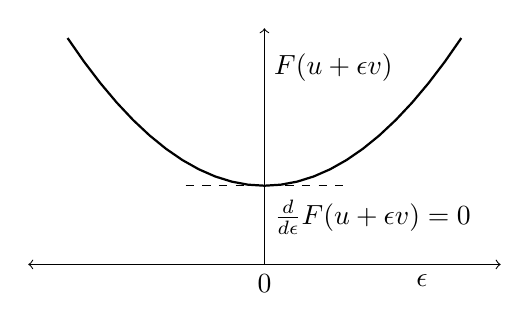
\begin{tikzpicture}
\draw[<->] ( -3,0) -- (3,0);
\draw[->] (0,0) --  (0,3);
\node at (2,0) [below] {$\epsilon$};
\node at (0,0) [below] {0};
\node at (0,2.5)[right]{$F(u + \epsilon v) $};

%\draw[thick,dashed] (-2.5,3) to [out=-60, in=180] (0,1) to [out=0, in=240] (2.5,3);
\draw[thick, domain=-2.5:2.5] plot ( \x, {1 + 0.3* \x*\x} );

\draw[dashed] (-1,1) -- +(2,0);
\node at (0,0.6) [right] {$\frac{d}{d \epsilon} F(u + \epsilon v) = 0$};
 
\end{tikzpicture}
\end{center}


\subsubsection*{Example: Energy Balance}

For example, consider film of soapy water suspended across an aperture.  At equilibrium, the soap film lies in the $x,y$ plane.  Let $u(x,y)$ be the the height of the film above the $x,y$ plane (at point ($x,y$)).

\begin{center}
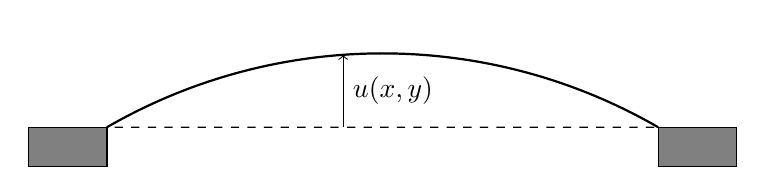
\begin{tikzpicture}

\draw [thick] (0,0) arc (120:60:7cm);
\draw (0,0) arc (120:60:7cm) [dashed] -- (0,0);

\draw [fill=gray] (0,0) rectangle ++(-1,-0.5);
\draw [fill=gray] (7,0) rectangle ++(1,-0.5);

\draw[->] (3,0) -- node[right]{$u(x,y)$} ++(0,0.92);

\end{tikzpicture}
\end{center}

Assume some force below the film distorts it, pushing it upwards.  The force does work on the soap film. If $f$ is the force on the film per unit area (pressure), then the work done moving an infinitesimal area element $dA$ a distance $u(x,y)$ is $dW = u f dA$. Thus the total work done on the soap film is the integral: 
\begin{equation}
W = \int_{\Omega} f u \,dA
\end{equation} 

\begin{center}
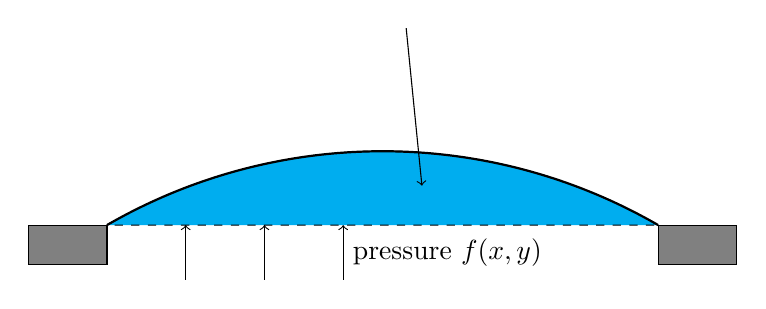
\begin{tikzpicture}

\draw [fill=cyan] (0,0) arc (120:60:7cm) [dashed] -- (0,0);
\draw [thick] (0,0) arc (120:60:7cm);

\draw [fill=gray] (0,0) rectangle ++(-1,-0.5);
\draw [fill=gray] (7,0) rectangle ++(1,-0.5);

\draw[<-] (3,0) -- node[right]{pressure $f(x,y)$} ++(0,-0.7);
\draw[<-] (1,0) -- ++(0,-0.7);
\draw[<-] (2,0) -- ++(0,-0.7);

\draw[<-] (4,0.5) -- ++(-0.2,2);
\end{tikzpicture}
\end{center}

The work done on the soap film is stored as elastic potential energy.  The soap film has a surface tension that acts tangentially to the surface.  A virtual length $dy$ has a force $2 \gamma dy$ acting perpendicularly to it. The force is \emph{constant,} so if the length is moved distance $dx$, creating new area $dxdy$, the work done is $ 2 \gamma dxdy$.  Thus, the change in potential energy is proportional to the change in area.

Consider a tangent plane of $u(x,y)$ located above an infinitesimal area element $dxdy$.  The tangent plane is bounded by the vectors $(dx,0,dx \partial_x u)$ and $(0,dy,dy \partial_y u)$. Their cross product is the normal vector to the plane\\
 $\vec{n} = (-dxdy \partial_x u, -dxdy \partial_y u, dxdy) $. The area of the infinitesimal tangent plane is equal to the magnitude of the normal vector:
\begin{equation}
dA = |\vec{n}| = dxdy \sqrt{1 + \partial_x u^2 + \partial_y u^2}
\end{equation}

For convenience, we use $|\nabla u|^2 = \nabla u \cdot \nabla u = \partial_x u^2 + \partial_y u^2  $.  The total area of the soap film is:
\begin{equation}
A =  \int_{\Omega} \sqrt{1 + |\nabla u|^2} \;dxdy
\end{equation}

If the soap bubble is distorted not too far from its equilibrium shape, then $\partial_x u \ll 1$ and $\partial_y u \ll 1$, so that:
\begin{equation}
\sqrt{1 + |\nabla u|^2} \approx \sqrt{1 + |\nabla u|^2 + \frac{1}{4} |\nabla u|^4}
= \sqrt{(1 + \frac{1}{2} |\nabla u|^2)^2}
= 1 + \frac{1}{2} |\nabla u|^2
\end{equation}
Then the \emph{change} in area from the equilibrium area is:
\begin{equation}
\int_{\Omega} 1 + \frac{1}{2} |\nabla u|^2 \;dxdy - \int_{\Omega} dxdy = 
\int_{\Omega} \frac{1}{2} |\nabla u|^2 \;dxdy
\end{equation}

Let $k$ be the surface tension coefficient.  Then the elastic potential energy is $k \frac{1}{2} \int_{\Omega}  |\nabla u|^2 \;dA $, and this is exactly equal to the work done on the soap film by the pressure:

\begin{equation}
k \frac{1}{2} \int_{\Omega} |\nabla u|^2 \;dA = \int_{\Omega} f u \;dA
\end{equation}

\vspace{1em}
\textbf{NOTE:}  This also models the energy balance of a deformed rubber membrane, \emph{if} the deformation is small enough that the tension is considered to be \emph{constant} throughout the deformation (rather than increasing linearly with area).

\vspace{2em}
We can express this as a functional to be minimized:
\begin{equation}
F(u) =  k \frac{1}{2} \int_{\Omega} |\nabla u|^2 \,dA - \int_{\Omega} f u \,dA
\end{equation}

And take the functional derivative:
\begin{align}
\frac{d}{d\epsilon}F & = \lim_{\epsilon \rightarrow 0}
                         \frac{F(u + \epsilon v) - F(u)}{\epsilon} \\
  & = \lim_{\epsilon \rightarrow 0}
    \frac{k \frac{1}{2} \int_{\Omega} |\nabla (u + \epsilon v)|^2 - |\nabla u|^2 \,dA
        - \int_{\Omega} f (u + \epsilon v) - f u \,dA}
         {\epsilon} \\
  & = \lim_{\epsilon \rightarrow 0}
    \frac{k \frac{1}{2} \int_{\Omega} |\nabla u + \epsilon \nabla v|^2 - |\nabla u|^2 \,dA
        - \int_{\Omega} f u + \epsilon f v - f u \,dA}
         {\epsilon} \\
  & = \lim_{\epsilon \rightarrow 0}
    \frac{k \frac{1}{2} \int_{\Omega} (\nabla u +  \epsilon \nabla v) \cdot 
    (\nabla u +  \epsilon \nabla v) - \nabla u \cdot \nabla u \,dA
        - \int_{\Omega} \epsilon f v \,dA}
         {\epsilon} \\       
  & = \lim_{\epsilon \rightarrow 0}
    \frac{k \frac{1}{2} \int_{\Omega} \nabla u \cdot \nabla u + 2 \epsilon \nabla u \cdot 
    \nabla v + \epsilon^2 \nabla v \cdot \nabla v - \nabla u \cdot \nabla u \,dA
        - \int_{\Omega} \epsilon f v \,dA}
         {\epsilon} \\                    
  & = \lim_{\epsilon \rightarrow 0}
    \frac{k \frac{1}{2} \int_{\Omega} 2 \epsilon \nabla u \cdot \nabla v
     + \epsilon^2 \nabla v \cdot \nabla v \,dA
        - \int_{\Omega} \epsilon f v \,dA}
         {\epsilon} \\
  & = \lim_{\epsilon \rightarrow 0}
    k \frac{1}{2} \int_{\Omega} 2 \nabla u \cdot \nabla v
     + \epsilon \nabla v \cdot \nabla v \,dA
        - \int_{\Omega} f v \,dA\\     
  & =
    k \int_{\Omega} \nabla u \cdot \nabla v \,dA
        - \int_{\Omega} f v \,dA
\end{align}

Thus the variational form $\frac{d}{d\epsilon}F = 0$ is:
\begin{equation}
k \int_{\Omega} \nabla u \cdot \nabla v \,dA
        - \int_{\Omega} f v \,dA = 0
\end{equation}

This relation is true for any \emph{almost} arbitrary variation $v$.  In fact, $v$ must be integrable on the domain $\Omega$, and its first derivatives must be integrable on $\Omega$.
The space of functions meeting these requirements is known as the Sobolev space $H^1(\Omega) $.  So formally, $v$ belongs to the Sobolev space:
\begin{equation}
v \in H^1 (\Omega)
\end{equation}
Moreover, because the value of $u$ is given at the boundary, $v$ must be zero at the boundary.  Formally, $v$ is in the Sobolev space:
\begin{equation}
v \in H_0^1 (\Omega)
\end{equation}

\subsection*{Alternative Route to Variational Form}

The point is that the variational form
\begin{equation}
k \int_{\Omega} \nabla u \cdot \nabla v \,dA  - \int_{\Omega} f v \,dA = 0
\qquad
\forall v \in H_0^1(\Omega)
\end{equation}
may be easier to solve than the original energy functional.

However, the variational form can be derived by other means.  In fact, there are variational formulations for which there is \emph{no} corresponding functional to minimize.  So in a sense the variational formulation is more fundamental than the calculus of variations.

We shall use this alternative derivation as part of our homogenization procedure.  We bootstrap by starting with the case of Stokes flow over a \emph{flat} surface.

\subsubsection*{Stokes Flow in Variational Form}

Before beginning, we recall a vector identity.  For scalars $g$ and $u$:
\begin{align*}
g \nabla^2 u & = g \partial_x^2 u + g \partial_y^2 u \\
\nabla u \cdot \nabla g & = \partial_x u \partial_x g + \partial_y u \partial_y g \\
\nabla \cdot (g \nabla u) & = \partial_x (g \partial_x u) + \partial_y (g \partial_y u) \\
  & = \partial_x u \partial_x g + g \partial_x^2 u + \partial_y u \partial_y g + g \partial_y^2 u \\ 
  & = \nabla u \cdot \nabla g + g \nabla^2 u 
\end{align*}
\begin{equation*}
\therefore \quad g \nabla^2 u = \nabla \cdot (g \nabla u) - \nabla u \cdot \nabla g
\end{equation*}

\vspace{2em}

On some domain $\Omega$, Stokes flow holds:
\begin{equation}
\nabla^2 u = \nabla p \qquad \text{on} \; \Omega
\end{equation}

\vspace{1em}
\begin{center}
\begin{tikzpicture}
\draw[dashed] (0,0) rectangle (4,2);

\node at (2,1) {$\Omega $};
\node at (4.5,1) {$\Gamma $};
\end{tikzpicture}
\end{center}

We introduce a \emph{test function} $g$, from the appropriate Sobolev space:  $g$ and its first derivatives are integrable on $\Omega$, and $g$ is zero on the boundary $\Gamma$.
\begin{equation}
g \in H_0^1(\Omega) \qquad (g=0 \; \text{on} \; \Gamma)
\end{equation}

We multiply the Stokes equation by the test function $g$:
\begin{equation}
g \nabla^2 u = g \nabla p
\end{equation}
and integrate over the domain $\Omega$.
\begin{equation}
\int_{\Omega} g \nabla^2 u = \int_{\Omega} g \nabla p
\end{equation}
then substitute $g \nabla^2 u = \nabla \cdot (g \nabla u) - \nabla u \cdot \nabla g$:
\begin{equation}
\int_{\Omega} \nabla \cdot (g \nabla u) - \nabla u \cdot \nabla g  
= \int_{\Omega} g \nabla p
\end{equation}
\begin{equation}
\int_{\Omega} \nabla \cdot (g \nabla u) - \int_{\Omega} \nabla u \cdot \nabla g  
= \int_{\Omega} g \nabla p
\end{equation}

\begin{equation}
\text{Recall the Divergence Theorem:} \qquad
\int_{\Omega} \nabla \cdot \vec{a}  = \int_{\Gamma} \vec{a} \cdot \vec{n}
\end{equation}
Therefore
\begin{equation}
\int_{\Omega} \nabla \cdot (g \nabla u) = 
\int_{\Gamma} (g \nabla u) \cdot \vec{b} = \int_{\Gamma} g (\nabla u \cdot \vec{n}
= \int_{\Gamma} g \frac{\partial u}{\partial n}
\end{equation}
Now the test function $g$ was defined to be zero on $\Gamma$, thus
\begin{equation}
\int_{\Omega} \nabla \cdot (g \nabla u)
 = \int_{\Gamma} g \frac{\partial u}{\partial n} =0
\end{equation}

This leaves finally:
\begin{equation}
- \int_{\Omega} \nabla u \cdot \nabla g  
= \int_{\Omega} g \nabla p
\end{equation}
which closely resembles the variational form derived from the energy functional.


\subsubsection*{Stokes Flow with Slip in Variational Form}

We now progress to the variational form for Stokes flow over a flat boundary with Navier slip.

On the domain $\Omega$, Stokes flow holds:
\begin{equation}
\nabla^2 u = \nabla p \qquad \text{on} \; \Omega
\end{equation}

Now the boundary of the entire domain, $\Gamma$, must be split up into the \emph{bottom} boundary $\Gamma_b$, and the rest of the boundary, $\Gamma_0$.  The bottom boundary $\Gamma_b$ is the solid surface with slip.  Thus, on $\Gamma_b$, Navier slip holds:
\begin{equation}
u = b \frac{\partial u}{\partial n} \qquad \text{on} \; \Gamma_b
\end{equation}

\vspace{1em}
\begin{center}
\begin{tikzpicture}
\draw (0,0) -- (4,0);
\draw[dashed] (0,0) -- ++(0,2) -| (4,0);

\node at (2,1) {$\Omega $};
\node at (2,-0.5) {$\Gamma_b$};
\node at (4.5,1) {$\Gamma_0 $};
\end{tikzpicture}
\end{center}



Now care must be taken to choose the appropriate function space for our test function.  As before, the  test function and its first derivatives must be integrable on $\Omega$.  
But now, $g$ must vanish on all of the boundary \emph{except} the bottom boundary $\Gamma_b$.

\begin{equation}
g \in H^1_{\Gamma_b} (\Omega) = \lbrace g \in H^1(\Omega): g = 0 \; \text{on}\; \Gamma_0 \rbrace 
\quad (g \neq 0 \; \text{on} \; \Gamma_b)
\end{equation}

Multiply  by $g$ and integrate over $\Omega$:
\begin{equation}
\int_{\Omega} g \nabla^2 u = \int_{\Omega} g \nabla p
\end{equation}

Ending up with
\begin{equation}
\int_{\Gamma} g \frac{\partial u}{\partial n}
 - \int_{\Omega} \nabla u \cdot \nabla g  
= \int_{\Omega} g \nabla p
\end{equation}
Now, $g=0$ on all of $\Gamma$ except the bottom boundary, so:
\begin{equation}
\int_{\Gamma} g \frac{\partial u}{\partial n}
= \int_{\Gamma_b} g \frac{\partial u}{\partial n}
\end{equation}
The slip condition on $\Gamma_b$ implies:
\begin{equation}
\frac{\partial u}{\partial n} = \frac{1}{b}u
\end{equation}
So we substitute this, to get our variational form:
\begin{equation}
\int_{\Gamma_b} g \frac{1}{b} u 
 - \int_{\Omega} \nabla u \cdot \nabla g  
= \int_{\Omega} g \nabla p
\end{equation}


\section*{Variational Form of Stokes Flow with Tensor Slip}

Before deriving the variational formulation of our full model of 3-D flow with tensorial slip, we recall various tensor identities.

\subsubsection*{Tensor Double Dot Product}

The double dot product of two tensors, also known as the Frobenius inner product, is a generalization of the vector inner product:

\begin{equation*}
A = 
\begin{bmatrix}
a & b \\
c & d
\end{bmatrix}
, \quad Z = 
\begin{bmatrix}
x & y \\
z & w
\end{bmatrix}
, \quad
A:Z = ax + by + cz + dw
\end{equation*}

As expected, addition distributes over this form of multiplication:
\begin{equation*}
(A + B):(Z + W) = A:Z + A:W + B:Z + B:W
\end{equation*}

\subsubsection*{Tensor Vector Divergence Identity}

For a tensor $T$ and vector $\vec{g}$:

\begin{equation*}
T:\nabla \vec{g} = T_{11}\partial_x g_x + T_{12}\partial_x g_y + T_{21}\partial_y g_x
+ T_{22} \partial_y g_y
\end{equation*}
and
\begin{equation*}
\nabla \cdot T = 
\begin{bmatrix}
\partial_x & , & \partial_y
\end{bmatrix}
\begin{bmatrix}
T_{11} & T_{12} \\
T_{21} & T_{22}
\end{bmatrix} =
\begin{bmatrix}
\partial_x T_{11} + \partial_y T_{21} &,& \partial_x T_{12} + \partial_y T_{22}
\end{bmatrix}
\end{equation*}
so that
\begin{equation*}
(\nabla \cdot T) \cdot \vec{g} = 
g_x \partial_x T_{11} + g_x \partial_y T_{21} + g_y \partial_x T_{12}
 + g_y \partial_y T_{22}
\end{equation*}
 Furthermore
\begin{equation*}
T \cdot \vec{g} = 
\begin{bmatrix}
T_{11} & T_{12} \\
T_{21} & T_{22}
\end{bmatrix}
\begin{bmatrix}
g_x \\
g_y
\end{bmatrix} = 
\begin{bmatrix}
T_{11} g_x + T_{12} g_y \\
T_{21} g_x + T_{22} g_y
\end{bmatrix}
\end{equation*}
Therefore
\begin{align*}
\nabla \cdot (T \cdot \vec{g}) & = 
\partial_x (T_{11} g_x) + \partial_x (T_{12} g_y) +
\partial_y (T_{21} g_x) + \partial_y (T_{22} g_y) \\
 & = g_x \partial_x T_{11} + \underbrace{T_{11} \partial_x g_x} +
     g_y \partial_x T_{12} + \underbrace{T_{12} \partial_x g_y} +
     g_x \partial_y T_{21} + \underbrace{T_{21} \partial_y g_x} +
     g_y \partial_y T_{22} + \underbrace{T_{22} \partial_y g_y} \\
 & = T:\nabla \vec{g} + (\nabla \cdot T) \cdot \vec{g}
\end{align*}

We have shown:
\begin{equation*}
\nabla \cdot (T \cdot \vec{g}) =  T:\nabla \vec{g} + (\nabla \cdot T) \cdot \vec{g}
\end{equation*}


\subsubsection*{Application to Velocity Gradient Tensor}

Substituting $T = \nabla \vec{u}$ in the identity gives:
\begin{equation*}
\nabla \cdot (\nabla \vec{u} \cdot \vec{g}) = 
\nabla \vec{u}:\nabla \vec{g} + (\nabla \cdot \nabla \vec{u}) \cdot \vec{g}
\end{equation*}
and the `vector Laplacian' is defined:
\begin{equation*}
\nabla \cdot \nabla \vec{u} =
\begin{bmatrix}
\partial_x \partial_x u + \partial_y \partial_y u &,& \partial_x \partial_x v + \partial_y \partial_y v
\end{bmatrix} =
\begin{bmatrix}
\nabla^2 u &,& \nabla^2 v
\end{bmatrix}
= \nabla^2 \vec{u}
\end{equation*}
So
\begin{equation*}
\nabla \cdot (\nabla \vec{u} \cdot \vec{g}) = 
\nabla \vec{u}:\nabla \vec{g} + \nabla^2 \vec{u} \cdot \vec{g}
\end{equation*}

Similarly for the transpose of the velocity gradient tensor:
\begin{equation*}
\nabla \cdot (\nabla \vec{u}^T \cdot \vec{g}) = 
\nabla \vec{u}^T:\nabla \vec{g} + (\nabla \cdot \nabla \vec{u}^T) \cdot \vec{g}
\end{equation*}
Now, however, the last term vanishes:
\begin{align*}
\nabla \cdot \nabla \vec{u} & =
\begin{bmatrix}
\partial_x \partial_x u + \partial_x \partial_y v &,&
 \partial_y \partial_x u + \partial_y \partial_y v
\end{bmatrix} \\
 & =
\begin{bmatrix}
\partial_x ( \partial_x u + \partial_y v ) &,&
\partial_y ( \partial_x u + \partial_y v )
\end{bmatrix} \\
 & = 
\begin{bmatrix}
\partial_x ( \nabla \cdot \vec{u}) &,&
\partial_y ( \nabla \cdot \vec{u})
\end{bmatrix} \\
 & = 
 \begin{bmatrix}
 0 &,& 0
 \end{bmatrix}
\end{align*}
since we assume the fluid is \textbf{incompressible}, so $\nabla \cdot \vec{u} = 0$ everywhere.

Thus
\begin{equation*}
\nabla \cdot (\nabla \vec{u}^T \cdot \vec{g}) = \nabla \vec{u}^T:\nabla \vec{g}
\end{equation*}

\subsubsection*{Deformation Rate Tensor Identity}

Extending our notation slightly to include vector fields other than $\vec{u}$, recall that the deformation rate tensor is:
\begin{equation*}
\mathbf{E}(\vec{u}) = \frac{\nabla \vec{u} + \nabla \vec{u}^T }{2}
\end{equation*}
so that:
\begin{equation*}
2 \mathbf{E}(\vec{g}) = \nabla \vec{g} + \nabla \vec{g}^T
\end{equation*}

Then the double dot product of two such tensors is:
\begin{align*}
2 \mathbf{E}(\vec{u}):2 \mathbf{E}(\vec{g}) & =
(\nabla \vec{u} + \nabla \vec{u}^T ):(\nabla \vec{g} + \nabla \vec{g}^T ) \\
4 \mathbf{E}(\vec{u}): \mathbf{E}(\vec{g}) & =
   \nabla \vec{u}:\nabla \vec{g} + \nabla \vec{u}:\nabla \vec{g}^T
 + \nabla \vec{u}^T:\nabla \vec{g} + \nabla \vec{u}^T: \nabla \vec{g}^T
\end{align*}
Now, transposition affects the double dot product such that \\
 $\nabla \vec{u}:\nabla \vec{g} =\nabla \vec{u}^T: \nabla \vec{g}^T$ 
 and $ \nabla \vec{u}^T:\nabla \vec{g} = \nabla \vec{u}:\nabla \vec{g}^T $ , so
\begin{align*}
4 \mathbf{E}(\vec{u}): \mathbf{E}(\vec{g}) & =
   2 \nabla \vec{u}:\nabla \vec{g} + 2 \nabla \vec{u}^T:\nabla \vec{g} \\
2 \mathbf{E}(\vec{u}): \mathbf{E}(\vec{g}) & =
   \nabla \vec{u}:\nabla \vec{g} + \nabla \vec{u}^T:\nabla \vec{g}   
\end{align*}

\vspace{1em}
Finally,
\begin{align*}
\nabla \cdot ( (\nabla \vec{u} + \nabla \vec{u}^T) \cdot \vec{g}) & =
\nabla \cdot ( \nabla \vec{u} \cdot \vec{g} + \nabla \vec{u}^T \cdot \vec{g}) \\
  & = \nabla \cdot ( \nabla \vec{u} \cdot \vec{g}) +
      \nabla \cdot ( \nabla \vec{u}^T \cdot \vec{g}) \\
  & = \nabla^2 \vec{u} \cdot \vec{g} + \nabla \vec{u}:\nabla \vec{g}
      + \nabla \vec{u}^T:\nabla \vec{g} \\
  & = \nabla^2 \vec{u} \cdot \vec{g} + 2 \mathbf{E}(\vec{u}):\mathbf{E}(\vec{g})
\end{align*}
Therefore:
\begin{equation*}
\nabla^2 \vec{u} \cdot \vec{g} = 
\nabla \cdot ( (\nabla \vec{u} + \nabla \vec{u}^T) \cdot \vec{g})
- 2 \mathbf{E}(\vec{u}):\mathbf{E}(\vec{g})
\end{equation*}


\subsection*{Variational Form of Stokes Flow with Tensor Slip}

We have a domain $\Omega$, the boundary of which is made up of two parts, $\Gamma_b$ and $\Gamma_0$.  On the domain $\Omega$ we have Stokes flow:
\begin{equation}
\nabla^2 \vec{u} = \frac{1}{\mu} \nabla p
\end{equation}
On the boundary $\Gamma_b$ we have the tensor slip condition:
\begin{equation}
\frac{1}{b} \vec{u} = (\nabla \vec{u} + \nabla \vec{u}^T)\cdot \vec{n}
\quad \text{or} \quad
\frac{1}{b} \vec{u} = 2 \mathbf{E}(\vec{u}) \cdot \vec{n}
\end{equation}

\vspace{1em}
\begin{center}
\begin{tikzpicture}

\draw [domain=0:4.5,samples=200] plot (\x,{ 0.2 * sin(7*\x r)} );
\draw[dashed] (0,0) -- ++(0,2) -| (4.5,0);

\node at (2.25,-0.5) {$\Gamma_b $};
\node at (5,1) {$\Gamma_0 $};
\node at (2.25,1) {$\Omega $};

\end{tikzpicture}
\end{center}

We introduce an arbitrary test function $\vec{g}$ from the appropriate Sobolev space.
\begin{equation}
\vec{g} \in H^1_{\Gamma_b}(\Omega) = 
\{ \vec{g} \in H^1(\Omega), \quad \vec{g}=0 \text{ on } \Gamma_0 \}
\end{equation}

We take the dot product of the Stokes PDE with $\vec{g}$:
\begin{equation}
\nabla^2 \vec{u} \cdot \vec{g} = \frac{1}{\mu} \nabla p \cdot \vec{g}
\end{equation}
and integrate over the domain:
\begin{equation}
\int_{\Omega} \nabla^2 \vec{u} \cdot \vec{g} = 
\frac{1}{\mu} \int_{\Omega}  \nabla p \cdot \vec{g}
\end{equation}

%%%%
%Consider the right hand side.  Recall that by integration by parts:
%\begin{equation}
%\frac{1}{\mu} \int_{\Omega}  \nabla p \cdot \vec{g} = 
%\frac{1}{\mu} \int_{\Omega} \nabla \cdot p\vec{g} - 
%\frac{1}{\mu} \int_{\Omega} p \nabla \cdot \vec{g}
%\end{equation}
%By the Divergence Theorem:
%\begin{equation}
%\frac{1}{\mu} \int_{\Omega} \nabla \cdot p\vec{g} =
%\frac{1}{\mu} \int_{\Gamma} p \vec{g} \cdot \vec{n} =
%\frac{1}{\mu} \int_{\Gamma_b} p \vec{g} \cdot \vec{n} +
%\frac{1}{\mu} \int_{\Gamma_0} p \vec{g} \cdot \vec{n}
%\end{equation}


%Thus we have
%\begin{equation}
%\int_{\Omega} \nabla^2 \vec{u} \cdot \vec{g} = 
%\frac{1}{\mu} \int_{\Omega}  \nabla p \cdot \vec{g}
%\end{equation}

Substitute $ \nabla^2 \vec{u} \cdot \vec{g} = \nabla \cdot ( 2 \mathbf{E}(\vec{u}) \cdot \vec{g}) - 2 \mathbf{E}(\vec{u}):\mathbf{E}(\vec{g}) $
\begin{equation}
\int_{\Omega} \nabla \cdot ( 2 \mathbf{E}(\vec{u}) \cdot \vec{g} ) - 
2 \int_{\Omega} \mathbf{E}(\vec{u}) : \mathbf{E}(\vec{g})  = 
\frac{1}{\mu} \int_{\Omega}  \nabla p \cdot \vec{g}
\end{equation}

By the Divergence Theorem:
\begin{equation}
\int_{\Omega} \nabla \cdot ( 2 \mathbf{E}(\vec{u}) \cdot \vec{g} ) =
\int_{\Gamma} ( 2 \mathbf{E}(\vec{u}) \cdot \vec{g} ) \cdot \vec{n}
\end{equation}
And $\mathbf{E}$ is symmetric, so:
\begin{equation}
\int_{\Gamma} ( 2 \mathbf{E}(\vec{u}) \cdot \vec{g} ) \cdot \vec{n} =
\int_{\Gamma} ( 2 \mathbf{E}(\vec{u})^T \cdot \vec{n} ) \cdot \vec{g} =
\int_{\Gamma} ( 2 \mathbf{E}(\vec{u}) \cdot \vec{n} ) \cdot \vec{g}
\end{equation}
The boundary integral can be split into separate integrals over $\Gamma_b$ and $\Gamma_0$.\begin{equation}
\int_{\Gamma} ( 2 \mathbf{E}(\vec{u}) \cdot \vec{n} ) \cdot \vec{g} =
\int_{\Gamma_b} ( 2 \mathbf{E}(\vec{u}) \cdot \vec{n} ) \cdot \vec{g} +
\int_{\Gamma_0} ( 2 \mathbf{E}(\vec{u}) \cdot \vec{n} ) \cdot \vec{g}
\end{equation}
Now, $\vec{g} = 0$ on $\Gamma_0$, so $ \int_{\Gamma_0} ( 2 \mathbf{E}(\vec{u}) \cdot \vec{n} ) \cdot \vec{g} $ vanishes.

While on $\Gamma_b$, the slip condition holds.
So we substitute the tensor slip boundary condition $ 2 \mathbf{E}(\vec{u}) \cdot \vec{n} = \frac{1}{b} \vec{u}$:
\begin{equation}
\int_{\Gamma_b} ( 2 \mathbf{E}(\vec{u}) \cdot \vec{n} ) \cdot \vec{g} =
\int_{\Gamma_b} \frac{1}{b} \vec{u} \cdot \vec{g}
\end{equation}
Therefore:
\begin{equation}
\int_{\Gamma} ( 2 \mathbf{E}(\vec{u}) \cdot \vec{n} ) \cdot \vec{g} =
\int_{\Gamma} \frac{1}{b} \vec{u} \cdot \vec{g}
\end{equation}
Thus:
\begin{equation}
\int_{\Omega} \nabla \cdot ( 2 \mathbf{E}(\vec{u}) \cdot \vec{g} ) =
\int_{\Gamma} \frac{1}{b} \vec{u} \cdot \vec{g}
\end{equation}

\vspace*{1em}
And the variational formulation for Stokes flow with tensor slip is:
\begin{equation}
\int_{\Gamma} \frac{1}{b} \vec{u} \cdot \vec{g} = 
2 \int_{\Omega} \mathbf{E}(\vec{u}) : \mathbf{E}(\vec{g}) +
\frac{1}{\mu} \int_{\Omega}  \nabla p \cdot \vec{g}
\end{equation}


\section*{Weak Convergence}

\subsubsection*{Sequence of Functions}

Consider a function, say $f(x) = \sin(x)$, with an additional parameter $n$, where $n$ is a positive integer.  For example:
\begin{equation}
f_n = \frac{1}{n} \sin (x)
\end{equation}
For each $n \in \mathbb{Z}$ we have a new function.  Thus we have a \emph{sequence} of functions, indexed by $n$.

\begin{center}
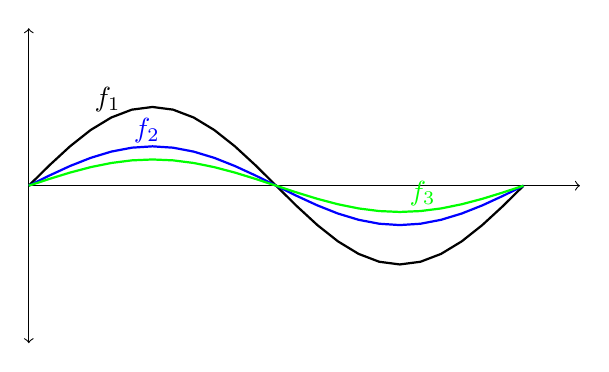
\begin{tikzpicture}

\draw[->] (0,0) -- (7,0);
\draw[<->] (0,-2) -- (0,2);

\draw [thick, domain=0:6.283] plot (\x, { sin(\x  r) });
\draw [color=blue,thick, domain=0:6.283] plot (\x, { sin(\x  r)/2 });
\draw [color=green,thick, domain=0:6.283] plot (\x, { sin(\x  r)/3 });

\node at (1,1.1) {$f_1$};
\node at (1.5,0.7) [color=blue] {$f_2$};
\node at (5,-0.1) [color=green] {$f_3$};

%\draw[color=red,thick, samples=97, domain=1:5] plot (\x, { 0.2 * sin( 3*pi*(\x-1) r) } );

\end{tikzpicture}
\end{center}

As $n \rightarrow \infty$, a sequence of functions may converge to a limit. 
A function $f_n$ in the sequence may be made arbitrarily `close to' the limit function, by simply making $n$ large enough. (All subsequent functions after $f_n$ are at least as close.)

The functions, and the limit function, are points in a function space.  We need to define a `distance' between two points, that is, the notion of a function being `close to' another function.

\subsubsection*{Strong Convergence}

In a vector space, the distance between two points $\vec{a}$ and $\vec{b}$ is found by finding the difference vector $\vec{b} - \vec{a}$, and calculating its length, the norm 
\begin{equation}
\lVert  \vec{b} - \vec{a} \rVert = \sqrt{(\vec{b} - \vec{a})\cdot (\vec{b} - \vec{a})}
\end{equation}
How do we extend this simple Pythagorean calculation to vectors of \emph{infinite} dimension? For the components $a_i$ of an infinite-dimensional vector, the index $i$ has an infinite domain, so the components can be thought of as a function $a(i)$ on a continuum. So the dot product $\vec{a} \cdot \vec{a}$ naturally extends to become the square integral:
\begin{equation}
\text{Inner Product } \vec{a} \cdot \vec{a} = \int \lvert a(x) \rvert^2 \;dx,
\quad \text{Norm } \lVert \vec{a} \rVert = \sqrt{\vec{a} \cdot \vec{a} }
\end{equation}

Coming from the other direction, the space of functions now has a natural inner product: $ \langle a,b \rangle = \int f \bar{g}\; dx $ which for $\langle a,a \rangle$ is the same as the square integral above.

The space of functions that are square-integrable, together with the inner product defined above, is the Lebesgue space $L^2$.  Our sequence of functions naturally live in this space.  We now have a natural notion of the `closeness' of a function to another: roughly speaking, the area \emph{between} the functions.

The function sequence \textbf{strongly converges} to the limit function $f$ if:
\begin{equation}
\lVert f_n - f \rVert \to 0 \qquad \text{as} \qquad n \to \infty
\end{equation}
Explicitly:
\begin{equation}
\int \lvert f_n - f \rvert^2 \;dx  \to 0 \qquad \text{as} \qquad n \to \infty
\end{equation}
This is notated:
\begin{equation}
f_n \to f
\end{equation}



\subsection*{Weak Convergence}

Consider a sequence of functions defined by:
\begin{equation}
f_n = \sin(n x)
\end{equation}

which looks like:
\begin{center}
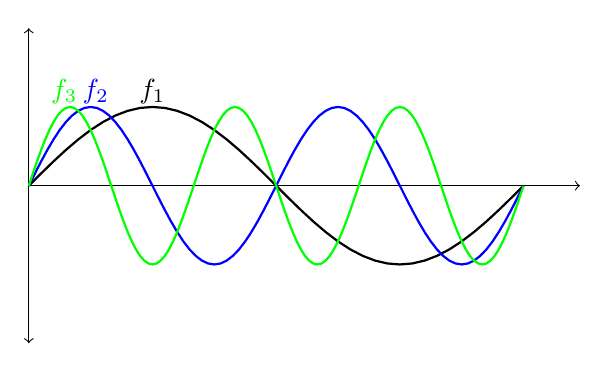
\begin{tikzpicture}

\draw[->] (0,0) -- (7,0);
\draw[<->] (0,-2) -- (0,2);

% samples = 4n per period + 1. n is resolution
\draw [thick, domain=0:6.283,samples=41] plot (\x, { sin(\x  r) });
\draw [color=blue,thick, domain=0:6.283, samples=81] plot (\x, { sin(2*\x  r) });
\draw [color=green,thick, domain=0:6.283, samples=121] plot (\x, { sin(3*\x r) });

\node at (1.57,1.2) {$f_1$};
\node at (0.85,1.2) [color=blue] {$f_2$};
\node at (0.45,1.2) [color=green] {$f_3$};

%\draw[color=red,thick, samples=97, domain=1:5] plot (\x, { 0.2 * sin( 3*pi*(\x-1) r) } );

\end{tikzpicture}
\end{center}

As $n$ increases, the period of the sine wave gets smaller and smaller, but the amplitude is unchanged.  In the limit as $n \to \infty$, the waveform gets infinitely `spiky'.  What does the sequence converge to?  There is no intuitive sense of the sinewave sequence getting `closer to' some limit function.  In fact, the sequence does not strongly converge.

However, there is a sense in which the function sequence converges. 

We multiply each function in the sequence by an arbitrary test function $g$, and integrate, thus creating a sequence of integrals:
\begin{equation}
\int g f_n \;dx
\end{equation}
If the integral sequence (strongly) converges to a limit integral:
\begin{equation}
\int g f_n \;dx \to \int g f \;dx
\end{equation}
then we say that $f_n$ \textbf{weakly converges} to $f$, and the `limit function' $f$ appearing in the limit integral is known as the \textbf{weak limit.}  This is also written:
\begin{equation}
f_n \rightharpoonup f
\end{equation}

What is the weak limit $f$?  If $f_n$ is a sequence of periodic functions (like our sine wave example) then $f$ is the \textbf{mean} of $fn$, denoted $\left< f_n \right>  $.

We shall prove (and use) this incredibly useful result.

\subsubsection*{Periodic Functions Weakly Converge to their Mean}

It is a `standard result' that periodic functions weakly converge to their mean.  In a 2002 paper \cite{Lukkassen2002}, Lukkassen and Wall state: ``We have not found proofs of [this] fact in the literature.  The aim of this paper is to present such proofs."  Their paper provides a rigorous proof (and generalization) of this proof.  Here, however, we present a simple intuitive proof, suitable for this thesis.

\vspace{1em}

Consider our example of a sine wave sequence, together with an arbitrary test function $g$, integrated over the domain $0$ to $2 \pi$.
Each integral in the sequence is of the form:
\begin{equation}
\int_0^{2\pi} g(x) \sin(nx) \;dx
\end{equation}
Over the domain $0$ to $2\pi$, the function $\sin(nx)$ has exactly $n$ periods, each of width $2\pi /n$.
We chop up the integral into $n$ separate integrals, each with a subdomain of width $2\pi/n$.
\begin{equation}
\sum_{k=1}^n  \int_{(k-1) \frac{2\pi}{n}}^{k \frac{2\pi}{n}} g(x) \sin(nx) \;dx
\end{equation}

\begin{center}
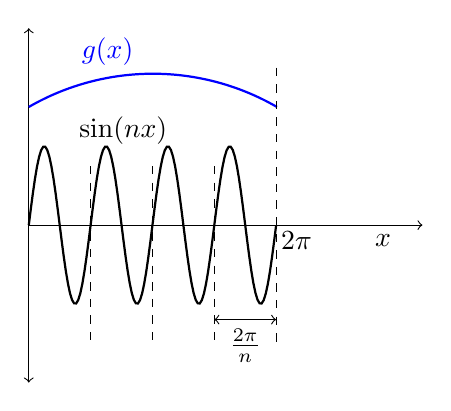
\begin{tikzpicture}

\draw[->] (0,0) -- (5,0);
\draw[<->] (0,-2) -- (0,2.5);
\node at (4.5,0) [below] {$x$};


% samples = 4n per period + 1. n is resolution
\draw [thick, domain=0:3.1416, samples=121] plot (\x, { sin(4*\x*2 r) });

\draw [color=blue, thick] (0,1.5) arc (120:60:3.1516 cm);

\node at (1.2,1.2) {$\sin(nx)$};
\node at (1,2.2) [color=blue] {$g(x)$};

\node at (3.4,-0.2) {$2\pi$};

\draw[dashed] (3.1416,2) -- ++(0,-3.5);
\foreach \k in {1,2,3}
{\draw[dashed] (\k*3.1416/4, 0.75) --++(0,-2.25);}

\draw[<->] (3.1416,-1.2) -- node[below] {$\frac{2\pi}{n}$} ++(-3.1416/4, 0);


\end{tikzpicture}
\end{center}

By a cunning change of variable, we `stretch' the domain so that in terms of the new variable, the period of the sine wave is again $2\pi$.  The domain is dilated by factor $n$ and now has width $2\pi n$.  The size of the integral will also increase by factor $n$, so we apply a $1/n$ correction.
\begin{equation}
\frac{1}{n} \sum_{k=1}^n  \int_{(k-1) 2\pi}^{k 2\pi} g \left(\frac{t}{n} \right) \sin(t) \;dt 
, \qquad x = \frac{t}{n}
\end{equation}

Put another way, we move the $n$ dependence from the sine function to the test function $g$.

\begin{center}
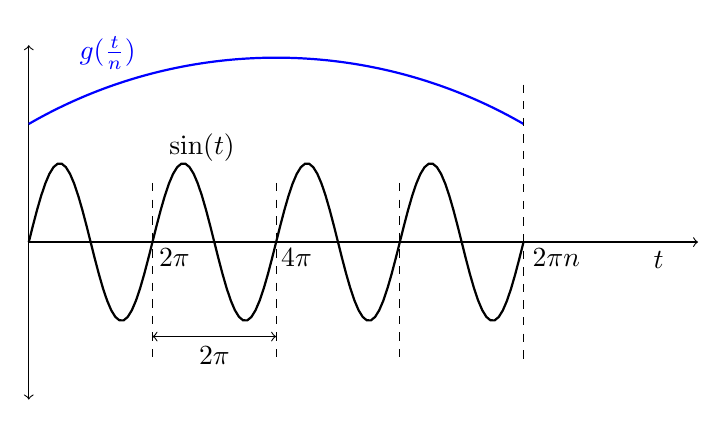
\begin{tikzpicture}

\draw[->] (0,0) -- (8.5,0);
\draw[<->] (0,-2) -- (0,2.5);
\node at (8,0) [below] {$t$};

% samples = 4n per period + 1. n is resolution
\draw [thick, domain=0:6.283, samples=121] plot (\x, { sin(4*\x r) });

\draw [color=blue, thick] (0,1.5) arc (120:60:6.283 cm);

\node at (2.2,1.2) {$\sin(t)$};
\node at (1,2.4) [color=blue] {$g(\frac{t}{n})$};

\node at (1.85,-0.2) {$2\pi$};
\node at (3.4,-0.2) {$4\pi$};
\node at (6.7,-0.2) {$2\pi n$};

\draw[dashed] (6.283,2) -- ++(0,-3.5);
\foreach \k in {1,2,3}
{\draw[dashed] (\k*3.1416/2, 0.75) --++(0,-2.25);}

\draw[<->] (3.1416,-1.2) -- node[below] {$2\pi$} ++(-3.1416/2, 0);


\end{tikzpicture}
\end{center}

Even more cunningly, we note that a period of $\sin(t)$ is the same for all $k$, so we use \emph{only} the integral from $0$ to $2\pi$, and `transport' the appropriate bit of $g(t)$ back to the interval $0$ to $2\pi$.  This is accomplished by adding $(k-1) (2\pi /n)$ to the argument of $g(t/n)$.  For clarity, we shall change variables again, $t \to \xi$, to highlight the fact that while the domain of $t$ is the interval $0$ to $2\pi n$, the domain of $\xi$ is only the interval $0$ to $2\pi$.
\begin{equation}
\frac{1}{n} \sum_{k=1}^n  \int_0^{2\pi} g\left(\frac{\xi}{n} + (k-1) \frac{2\pi}{n} \right) \sin(\xi) \;d\xi , \qquad x = \frac{\xi}{n}
\end{equation}

\begin{center}
\begin{tikzpicture}

\draw[->] (0,0) -- (8.5,0);
\draw[<->] (0,-2) -- (0,2.5);
\node at (8,0) [below] {$\xi$};

% samples = 4n per period + 1. n is resolution
\draw [thick, domain=0:1.5708, samples=32+1] plot (\x, { sin(4*\x r) });

\draw [dashed,color=blue, thick] (0,1.5) arc (120:60:6.283 cm);
\draw [color=blue, thick] (0,1.5) arc (120:104:6.283 cm);

\node at (0.7,1.2) {$\sin(\xi)$};
\node at (1,2.4) [color=blue] {$g(\frac{\xi}{n})$};

\node at (1.85,-0.2) {$2\pi$};
%\node at (3.4,-0.2) {$4\pi$};
%\node at (6.7,-0.2) {$2\pi n$};

%\draw[dashed] (1.5708,2) -- ++(0,-3.5);
%\draw[dashed] (6.283,2) -- ++(0,-3.5);
\foreach \k in {1,2,3,4}
{\draw[dashed] (\k*3.1416/2, 2.5) --++(0,-3);}

%\draw[<->] (3.1416,-1.2) -- node[below] {$2\pi$} ++(-3.1416/2, 0);


\end{tikzpicture}
\end{center}

So we have:
\begin{equation}
\frac{1}{n}   \int_0^{2\pi} g\left(\frac{\xi}{n}\right) \sin(\xi) \;d\xi
 + \frac{1}{n}   \int_0^{2\pi} g\left(\frac{\xi + 2\pi}{n} \right) \sin(\xi) \;d\xi
 + \cdots
\end{equation}
The sum can go under a single integral sign:
\begin{equation}
\frac{1}{n}
\int_0^{2\pi} g\left(\frac{\xi}{n}\right) \sin(\xi)
 + g\left(\frac{\xi + 2\pi}{n} \right) \sin(\xi) 
 + g\left(\frac{\xi + 4\pi}{n} \right) \sin(\xi) + \cdots \;d\xi
\end{equation}
And multiplication distributes over addition, so this is:
\begin{equation}
\frac{1}{n} \int_0^{2\pi} \sin(\xi)
\left[
g\left(\frac{\xi}{n} \right) + g\left(\frac{\xi + 2\pi}{n} \right)  +  
g\left(\frac{\xi + 4\pi}{n} \right) + \cdots 
\right] \;d\xi
\end{equation}
Or:
\begin{equation}
\frac{1}{n} \int_0^{2\pi} \sin(\xi)
 \sum_{k=1}^n g\left(\frac{\xi + (k-1) 2\pi}{n} \right) \;d\xi
\end{equation}
For later convenience, introduce a $2\pi$ and shift the $1/n$ factor:
\begin{equation}
\frac{1}{2\pi} \int_0^{2\pi} \sin(\xi) \;
 \sum_{k=1}^n g\left(\frac{\xi + (k-1) 2\pi}{n} \right) \frac{2\pi}{n} \;d\xi
 \end{equation}

What happens as $n \to \infty$?  The summation term can be written:
\begin{equation}
\sum_{k=1}^n g\left((k-1)\frac{ 2\pi}{n} + \frac{\xi}{n} \right) \frac{2\pi}{n}
 \end{equation}
Since $\xi$ is between $0$ and $2\pi$, the $\xi/n$ term is between $0$ and $2\pi/n$.
As $k$ ranges from $1$ to $n$, the $g(k)$ term provides $n$ `samples' of the function at discrete points a distance $2\pi/n$ apart, with the starting point offset from $0$ by the amount $\xi/n$.  Each sample $g(k)$ is multiplied by the width of the inter-sample distance, giving $n$ rectangles to sum up.   In the limit $n \to \infty$, this is one definition of the Riemann integral of $g$ over the interval $2\pi$.
\begin{equation}
\lim_{n \to \infty} \sum_{k=1}^n g\left((k-1)\frac{ 2\pi}{n} + \frac{\xi}{n} \right) \frac{2\pi}{n} = \int_0^{2\pi} g(x) \;dx
 \end{equation}

\begin{center}
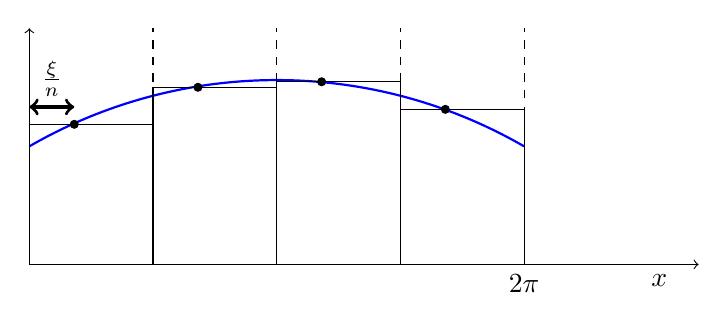
\begin{tikzpicture}
\draw[->] (0,0) -- (8.5,0);
\draw[->] (0,0) -- (0,3);
\node at (8,0) [below] {$x$};
\node at (6.283,0)[below] {$2\pi$};

\draw [color=blue, thick] (0,1.5) arc (120:60:6.283 cm);

\foreach \k / \y in {1 /1.78, 2/2.25, 3/2.32, 4/1.97}
{\draw[dashed] (\k*3.1416/2, 0) -- ++(0,3);
\draw (\k*3.1416/2,\y) rectangle (\k*3.1416/2 - 3.1416/2,0);
\draw[fill] (\k*3.1416/2 - 1, \y) circle (0.5mm); }

\draw[<->,very thick] (0,2) -- node[above]{$\frac{\xi}{n}$} ++(0.571,0);

\end{tikzpicture}
\end{center}


Thus we have:
\begin{equation}
\frac{1}{2\pi} \int_0^{2\pi} \sin(\xi)
\int_0^{2\pi} g(x) \;dx \;d\xi
= 
\left( \frac{1}{2\pi} \int_0^{2\pi} \sin(\xi) \;d\xi \right)
\left( \int_0^{2\pi} g(x) \;dx \right)
 \end{equation}
Now the integral with the sine function defines the \textbf{mean} of a function:
\begin{equation}
\left< \sin(x) \right> = \frac{1}{2\pi} \int_0^{2\pi} \sin(\xi) \;d\xi
\end{equation}
Therefore, we have shown that:
\begin{equation}
\lim_{n \to \infty} \int_0^{2\pi} g(x) \sin(nx) \;dx = \left< \sin(x) \right>
 \int_0^{2\pi} g(x) \;dx
\end{equation}
Or:
\begin{equation}
\int_0^{2\pi} g(x) \sin(nx) \;dx  \to  
 \int_0^{2\pi} g(x) \left< \sin(x) \right> \;dx
\end{equation}

The mean of $\sin(x)$ happens to be zero, so the limit vanishes.  But the foregoing argument holds for \emph{any} periodic function.  Therefore we have shown that \textbf{periodic functions weakly converge to their mean:}
\begin{equation}
\int g f_n \;dx \to \int g \left< f \right> \;dx
\end{equation}


\section*{Homogenizing the Variational Form}

We are now ready to homogenize our variational form:
\begin{equation}
\int_{\Gamma} \frac{1}{b} \vec{u} \cdot \vec{g} = 
2 \int_{\Omega} \mathbf{E}(\vec{u}) : \mathbf{E}(\vec{g}) +
\frac{1}{\mu} \int_{\Omega}  \nabla p \cdot \vec{g}
\end{equation}

The key concept is to model the slip boundary as a periodic function, and to set up a sequence of such functions, thus creating a sequence of boundaries.
\vspace{1em}

The physical boundary is a periodic function $h(x,y)$.  (For simplicity we shall illustrate it as a sine function, but it need not be.)  

The slip length is a periodic function $b(x,y)$ with the \textbf{same period} as $h(x,y)$.

\vspace{1em}
Define a sequence of surface functions by:
\begin{equation}
h_n = \frac{1}{n} h(nx, ny)
\end{equation}
Then as $n$ increases, the period and amplitude reduce by the \textbf{same factor.}  This is important -- it keeps the slope unchanged.

Similarly, define a sequence of slip functions by:
\begin{equation}
b_n = b(nx,ny)
\end{equation}
In this case, as $n$ increases, the period shortens, but the amplitude does \textbf{not} decrease.  This is physically correct -- the local slip length is an intrinsic property of the material, unaffected by scale.

For each $n$, there is a function $h_n$ describing the surface, and a function $b_n$ describing the intrinsic slip length on that surface.  Thus we have a sequence of boundaries, $\Gamma_n$.
Now, because $h_n$ reduces in amplitude with increasing $n$:
\begin{equation}
h_n \to 0, \qquad \text{as} \qquad n \to \infty
\end{equation}
Thus the sequence of boundaries (strongly) converges to the flat $x,y$ plane.

\begin{center}
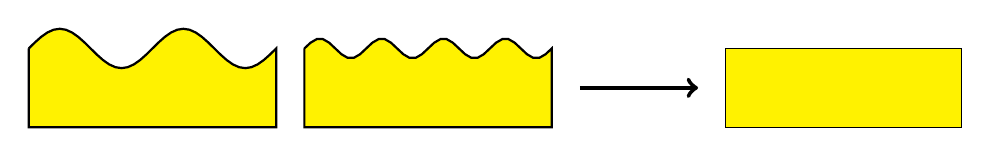
\begin{tikzpicture}
%\draw [thick, domain=0:6.283,samples=41] plot (\x, { sin(\x  r) });

\draw [fill=yellow, thick, domain=0:3.1416,samples=41] plot (\x, { sin(4*\x  r)/4 })
 |- (0,-1) -- (0,0);

\draw [fill=yellow, thick, domain=0:3.1416,samples=41] plot (\x+3.5, { sin(8*\x  r)/8 })
 |- (3.5,-1) -- (3.5,0);

\draw[->, ultra thick] (7,-0.5) -- ++(1.5,0);

\draw[fill=yellow] (8.85,0) rectangle ++(3,-1);

\end{tikzpicture}
\end{center}

\subsubsection*{Slip Integral}

Let us look more closely at the slip integral.  The integral is over a surface; each infinitesimal area element $dA$ is the area of the tangent plane to $h(x,y)$. Specifically:
\begin{equation}
dA = \sqrt{1 + \lvert \nabla h \rvert^2} \;dxdy
\end{equation}
Furthermore, the velocity function on the boundary is $\vec{u}(x,y,h)$.  Similarly, for the test function $\vec{g}(x,y,h)$.
Therefore, the slip integral is explicitly:
\begin{equation}
\int_{\Gamma} \frac{1}{b} \vec{u} \cdot \vec{g} \;dA =
\int_{\Gamma} \frac{1}{b(x,y)} \vec{u}(x,y,h) \cdot \vec{g}(x,y,h) 
\;\sqrt{1 + \lvert \nabla h \rvert^2} \;dxdy
\end{equation}

We insert the boundary sequence into the slip integral, giving:
\begin{equation}
\int_{\Gamma_n} \frac{\sqrt{1 + \lvert \nabla h_n \rvert^2}}{b_n} \;
 \vec{u}(x,y,h_n) \cdot \vec{g}(x,y,h_n) \;dxdy
\end{equation}

We now have a sequence of integrals.  This implies that we have a sequence of velocity solutions.  Since the boundary converges to the flat $x,y$ plane:
\begin{equation}
\vec{u}_n(x,y,h_n) \to \vec{u}(x,y,0), \qquad \vec{g}_n(x,y,h_n) \to \vec{g}(x,y,0)
\qquad \text{as} \qquad n \to \infty
\end{equation}

Now, while $h_n$ converges to the flat plane, it is constructed such that its partial derivatives in $\nabla h_n$ remain unchanged with increasing $n$.
Thus the the magnitude of $\sqrt{1 + \lvert \nabla h_n \rvert^2}$ does not change with increasing $n$ --- the function simply gets `spikier' as the period reduces.
The slip function $b_n$ is constructed to exhibit the same behaviour: unchanging amplitude with decreasing period.
Therefore, the compound function $\sqrt{1 + \lvert \nabla h_n \rvert^2} /b_n$ exhibits this common behaviour, getting spikier with increasing $n$.
As shown previously, these sorts of functions weakly converge to their mean:
\begin{equation}
\int_{\Gamma_n} \frac{\sqrt{1 + \lvert \nabla h_n \rvert^2}}{b_n} \;
\vec{g}\;dxdy \to
\int_{\Gamma} \left< \frac{\sqrt{1 + \lvert \nabla h \rvert^2}}{b} \right> \;
\vec{g} \;dxdy
\end{equation}

We add the velocity term $\vec{u}(x,y,h_n)$ to the above weak integral, to get the full slip integral.  
We would expect the velocity term to strongly converge to a single \emph{constant} velocity on the flat limit boundary.  Therefore, the integrand still exhibits the `spiky' behaviour, and still weakly converges to its mean:
\begin{equation}
\int_{\Gamma_n} \frac{\sqrt{1 + \lvert \nabla h_n \rvert^2}}{b_n} \;
\vec{u} \cdot \vec{g}\;dxdy \to
\int_{\Gamma} \left< \frac{\sqrt{1 + \lvert \nabla h \rvert^2}}{b} \right> \;
\vec{u} \cdot \vec{g} \;dxdy
\end{equation}

\subsubsection*{Volume Integrals}

As the boundary changes, the domain $\Omega$ changes shape slightly also, giving a sequence of domains $\Omega_n$.  Therefore we have a sequence of volume integrals.  Thus, finally, we have a sequence of variational formulations:

\begin{equation}
\int_{\Gamma_n} \frac{\sqrt{1 + \lvert \nabla h_n \rvert^2}}{b_n} \;
\vec{u} \cdot \vec{g}\;dxdy = 
2 \int_{\Omega_n} \mathbf{E}(\vec{u}) : \mathbf{E}(\vec{g}) +
\frac{1}{\mu} \int_{\Omega_n}  \nabla p \cdot \vec{g}
\end{equation}

which strongly converges to:
\begin{equation}
\int_{\Gamma} \left< \frac{\sqrt{1 + \lvert \nabla h \rvert^2}}{b} \right> \;
\vec{u} \cdot \vec{g} \;dxdy = 
2 \int_{\Omega} \mathbf{E}(\vec{u}) : \mathbf{E}(\vec{g}) +
\frac{1}{\mu} \int_{\Omega}  \nabla p \cdot \vec{g}
\end{equation}


Let us pause for a moment to gaze in awe at this limit variational formulation, and reflect on its significance.  By reversing the derivation shown earlier,
 we would arrive back at the classical formulation with
\begin{equation}
\nabla^2 \vec{u} = \frac{1}{\mu} \nabla p
\end{equation}
on the domain, while on the boundary $\Gamma_b$ we would have the tensor slip condition:
\begin{equation}
\left< \frac{\sqrt{1 + \lvert \nabla h \rvert^2}}{b} \right> \vec{u} = 2 \mathbf{E}(\vec{u}) \cdot \vec{n}
\end{equation}

This slip boundary condition defines our effective slip length:
\begin{equation}
\beff = \left< \frac{\sqrt{1 + \lvert \nabla h \rvert^2}}{b} \right> ^{-1}
\end{equation}

This is the central result of this thesis.

\subsection*{Interpretation}
Note that $\int_{\Omega} \sqrt{1 + \lvert \partial_x h \rvert^2} \; dx$ is the \textbf{arc length} of the function $h$ over the domain $\Omega$.  Extending to a three-dimensional surface,  $\int_{\Omega} \sqrt{1 + \lvert \nabla h \rvert^2} \; dxdy$ is the area of the surface function $h(x,y)$.

Hence, our effective slip is the \textbf{harmonic mean} of the local slip length, \textbf{weighted} by the fluid-solid contact area.


\begin{center}
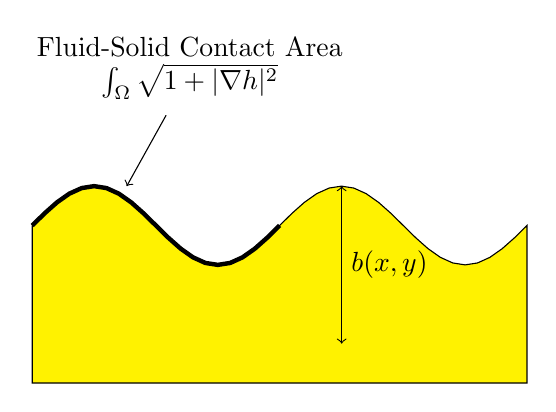
\begin{tikzpicture}

%samples = 4n per period + 1
\draw [fill=yellow, domain=0:6.283,samples=41] plot (\x, {sin(2*\x  r)/2 })
 |- ++(0,-2) -| (0,0); 
\draw [ultra thick, domain=0:3.1416,samples=21] plot (\x, {sin(2*\x  r)/2 });

\node at (2,2) [align=center]{Fluid-Solid Contact Area\\ $\int_{\Omega} \sqrt{1 + \lvert \nabla h \rvert^2} $};
\draw [<-] (1.2,0.5) -- ++(0.5,0.9);

\draw[<->] (3.93,0.5) -- node[right] {$b(x,y)$} ++(0,-2);

\end{tikzpicture}
\end{center}

If the surface is flat, then $\beff$ is simply the harmonic mean of the intrinsic slip length:
\begin{equation}
\beff = \left< \frac{1}{b} \right> ^{-1}
\end{equation}

If the surface is a flat \textbf{binary} surface, comprising discrete areas of high-slip surface and low-slip surface, with high-slip regions occupying fraction $\phi$ of the surface, then:
\begin{equation}
\beff = \left[ \phi \frac{1}{ b_{\mathrm{high}} }  + (1 -\phi) \frac{1}{ b_{\mathrm{low}}} \right]^{-1}
\end{equation}
as first proposed by Cecile Cottin-Bizonne \emph{et al} in 2004.


\subsection*{Applicability}

The effective slip length derived via homogenization is the \textbf{limiting} slip length as the period of the surface variation tends to zero.  A real surface obviously has a finite period of surface variation.  The effective slip length can in principle be measured experimentally.  

The critical question is:

\vspace{1em}
For what range of surfaces is the homogenized slip length a good approximation to the measured slip length?

\vspace{1em}
Equivalently, when is the flow over a rough, heterogeneous surface \textbf{close to} the flow over an effective homogenized surface?  

One approach to answer this is to ask: when is a rough surface close to the limit surface?  A reasonable answer is: when the \textbf{period is small compared to other length scales.}
The only other length scale is the intrinsic slip length.  Therefore, we propose that our $\beff$ is valid when the \textbf{minimum} intrinsic slip length is large compared to the period.

\begin{equation}
L \ll \min(b(x,y))
\end{equation}

In practice --- specifically, in our numerical testing --- our expression performs much better than that: we find that our $\beff$ approximates the measured effective slip length very well even when the minimum slip length is the same magnitude as the period.
(Details follow in a subsequent chapter.)




%\begin{center} \vspace{3em} \Coffeecup \end{center}

\bibliography{Lund_Thesis.bib}
\bibliographystyle{plain}

\end{document}



